%!TEX program = xelatex

\documentclass[11pt,titlepage]{report}
%!TEX root = main.tex

\usepackage[T1]{fontenc}
\usepackage{lmodern}
\usepackage[svgnames]{xcolor}
\usepackage{fontspec} % XeLaTeX required!
\usepackage{graphicx}
\usepackage{circuitikz}
\usepackage{tikz}
\usepackage{pifont}
\usepackage[some]{background}
\usepackage{xltxtra} 
\usepackage{setspace}
\usepackage[absolute]{textpos}
\usepackage[latin1]{inputenc}
\usepackage[english]{babel}
\usepackage{graphicx}
\usepackage{wrapfig}
\usepackage{fullpage}
\usepackage[margin=1in]{geometry}
\usepackage{float}
\usepackage{url}
\usepackage{multicol}
\usepackage{hyperref}
\usepackage{titlepic}
\usepackage{standalone}
\usepackage{siunitx}
\usepackage{booktabs}
\usepackage{amsmath}
\usepackage{unicode-math}
\usepackage{verbatim}
\usepackage{enumitem}
\usepackage{listings}
\usepackage{multirow}
\usepackage{pgfplots}
\pgfplotsset{compat=1.8}
\usepackage{caption} 
\usepackage[parfill]{parskip}
\usepackage{import}
\usepackage[backend=bibtexu,texencoding=utf8,bibencoding=utf8,style=ieee,sortlocale=en_GB,language=auto]{biblatex}
\usepackage[strict,autostyle]{csquotes}
\usepackage[final]{pdfpages}
\usepackage{subcaption}
\usepackage{ifplatform}
%\captionsetup[table]{skip=10pt}


% Fix for includepdf bug in Mac OS X
\newcommand{\insertpdfpath}[1]{
	\ifwindows
	\newcommand{\insertpdf}[2]{\includepdf[pages=##1]{##2}}
	\else
	\newcommand{\insertpdf}[2]{\includepdf[pages=##1]{#1/##2}}
	\fi
}

%set fonts
\setmainfont[Ligatures=TeX]{Myriad Pro}
\setmathfont{Asana Math}
\setmonofont{Lucida Console}

\usepackage{titlesec, color}
\renewcommand{\familydefault}{\sfdefault} %set font family
\renewcommand{\arraystretch}{1.2} %set table vertical spacing
\setlength\parindent{0pt} %no paragraph indent
\hypersetup{ %setup hyperlinks
    colorlinks,
    citecolor=black,
    filecolor=black,
    linkcolor=black,
    urlcolor=black
}

%redesign chapter headings
\definecolor{gray75}{gray}{0.75}
\newcommand{\chapternumber}{\thechapter}
\newcommand{\hsp}{\hspace{20pt}}
\titleformat{\chapter}[hang]{\Huge\bfseries}{\chapternumber\hsp\textcolor{gray75}{|}\hsp}{0pt}{\Huge\bfseries}

%Redefine appendix headers
\renewcommand{\appendixname}{Appendix}
\renewcommand{\appendixtocname}{Appendices}
\renewcommand{\appendixpagename}{Appendices}

%For code listings
\definecolor{black}{rgb}{0,0,0}
\definecolor{browntags}{rgb}{0.65,0.1,0.1}
\definecolor{bluestrings}{rgb}{0,0,1}
\definecolor{graycomments}{rgb}{0.4,0.4,0.4}
\definecolor{redkeywords}{rgb}{1,0,0}
\definecolor{bluekeywords}{rgb}{0.13,0.13,0.8}
\definecolor{greencomments}{rgb}{0,0.5,0}
\definecolor{redstrings}{rgb}{0.9,0,0}
\definecolor{purpleidentifiers}{rgb}{0.01,0,0.01}


\lstdefinestyle{csharp}{
language=[Sharp]C,
showspaces=false,
showtabs=false,
breaklines=true,
showstringspaces=false,
breakatwhitespace=true,
escapeinside={(*@}{@*)},
columns=fullflexible,
commentstyle=\color{greencomments},
keywordstyle=\color{bluekeywords}\bfseries,
stringstyle=\color{redstrings},
identifierstyle=\color{purpleidentifiers},
basicstyle=\ttfamily\small}

\lstdefinestyle{c}{
language=C,
showspaces=false,
showtabs=false,
breaklines=true,
showstringspaces=false,
breakatwhitespace=true,
escapeinside={(*@}{@*)},
columns=fullflexible,
commentstyle=\color{greencomments},
keywordstyle=\color{bluekeywords}\bfseries,
stringstyle=\color{redstrings},
identifierstyle=\color{purpleidentifiers},
}

\lstdefinestyle{matlab}{
language=Matlab,
showspaces=false,
showtabs=false,
breaklines=true,
showstringspaces=false,
breakatwhitespace=true,
escapeinside={(*@}{@*)},
columns=fullflexible,
commentstyle=\color{greencomments},
keywordstyle=\color{bluekeywords}\bfseries,
stringstyle=\color{redstrings},
identifierstyle=\color{purpleidentifiers}
}

\lstdefinestyle{vhdl}{
language=VHDL,
showspaces=false,
showtabs=false,
breaklines=true,
showstringspaces=false,
breakatwhitespace=true,
escapeinside={(*@}{@*)},
columns=fullflexible,
commentstyle=\color{greencomments},
keywordstyle=\color{bluekeywords}\bfseries,
stringstyle=\color{redstrings},
identifierstyle=\color{purpleidentifiers}
}

\lstdefinestyle{xaml}{
language=XML,
showspaces=false,
showtabs=false,
breaklines=true,
showstringspaces=false,
breakatwhitespace=true,
escapeinside={(*@}{@*)},
columns=fullflexible,
commentstyle=\color{greencomments},
keywordstyle=\color{redkeywords},
stringstyle=\color{bluestrings},
tagstyle=\color{browntags},
morestring=[b]",
  morecomment=[s]{<?}{?>},
  morekeywords={xmlns,version,typex:AsyncRecords,x:Arguments,x:Boolean,x:Byte,x:Char,x:Class,x:ClassAttributes,x:ClassModifier,x:Code,x:ConnectionId,x:Decimal,x:Double,x:FactoryMethod,x:FieldModifier,x:Int16,x:Int32,x:Int64,x:Key,x:Members,x:Name,x:Object,x:Property,x:Shared,x:Single,x:String,x:Subclass,x:SynchronousMode,x:TimeSpan,x:TypeArguments,x:Uid,x:Uri,x:XData,Grid.Column,Grid.ColumnSpan,Click,ClipToBounds,Content,DropDownOpened,FontSize,Foreground,Header,Height,HorizontalAlignment,HorizontalContentAlignment,IsCancel,IsDefault,IsEnabled,IsSelected,Margin,MinHeight,MinWidth,Padding,SnapsToDevicePixels,Target,TextWrapping,Title,VerticalAlignment,VerticalContentAlignment,Width,WindowStartupLocation,Binding,Mode,OneWay,xmlns:x}
}

\lstdefinestyle{matlab}{
language=Matlab,
showspaces=false,
showtabs=false,
breaklines=true,
showstringspaces=false,
breakatwhitespace=true,
escapeinside={(*@}{@*)},
columns=fullflexible,
commentstyle=\color{greencomments},
keywordstyle=\color{bluekeywords}\bfseries,
stringstyle=\color{purpleidentifiers},
identifierstyle=\color{purpleidentifiers}
}

%defaults
\lstset{
basicstyle=\ttfamily\small,
extendedchars=false,
numbers=left,
numberstyle=\ttfamily\tiny,
stepnumber=1,
tabsize=4,
numbersep=5pt
}
\addbibresource{../../library/bibliography.bib}

\begin{document}

\chapter{Assignment 1}
\section{Car model}
\begin{figure}[H]
	\centering
	\begin{tikzpicture}[node distance=2cm]
		\bgComponentNoBond{Se}{$S_e:u$}
		\bgComponent{}{1-1}{1}{right of=}{Se}{inbond}
		\bgComponent{}{mass}{$I:m$}{above of=}{1-1}{inbond}
		\bgComponent{}{res}{$R:\rho$}{right of=}{1-1}{inbond}
	\end{tikzpicture}
	\caption{Bond graph representation of the car model}
	\label{fig:ass-1-bond-simple}
\end{figure}

The second-order state-space model fitting the bond graph drawn in Figure~\ref{fig:ass-1-bond-simple} is given by

\begin{align}
	\dot{\vec{x}} = \frac{d}{dt}
	\begin{bmatrix}
		q_m \\
		f_m
	\end{bmatrix} &= \mat{A} \vec{x} + \mat{B} \vec{u} =
	\begin{bmatrix}
		0 & 1 \\
		0 & -\frac{\rho}{m}
	\end{bmatrix}
	\begin{bmatrix}
		q_m \\
		f_m
	\end{bmatrix} +
	\begin{bmatrix}
		0 \\
		\frac{1}{m}
	\end{bmatrix} u, \\
	\vec{y} = q_m &= \mat{C} \vec{x} + \mat{D} \vec{u} =
	\begin{bmatrix}
		1 & 0
	\end{bmatrix}
	\begin{bmatrix}
		q_m \\
		f_m
	\end{bmatrix}.
\end{align}

The eigenvalues with corresponding eigenvectors of our state-space model are

\begin{equation}
	\lambda_1 = 0\text{ with }
	\vec{v}_1 = \begin{bmatrix}
		1 \\
		0
	\end{bmatrix}\text{ and}
\end{equation}

\begin{equation}
	\lambda_2 = -\frac{\rho}{m}\text{ with }
	\vec{v}_2 = \begin{bmatrix}
		-\frac{m}{\rho} \\
		1
	\end{bmatrix}.
\end{equation}

Since we have two independent eigenvectors, $\lambda_2 < 0$ and $\lambda_1 = 0$, our system is marginally stable. To investigate the controllability and observability of a one-dimensional output system, we used the fact that a pair $(\mat{A},\mat{B})$ is controllable if $\mat{V}$ is a square matrix whose colums consist of different eigenvectors of $\mat{A}$, and every element of the vector $\mat{V}^{-1} \mat{B}$ is non-zero. If an element was to be zero, then the controllability matrix can not have full rank. Since

\begin{equation}
	\left[\vec{v}_1 \vec{v}_2 \right]^{-1} \mat{B} = \begin{bmatrix}
		\frac{1}{m} \\
		\frac{1}{\rho}
	\end{bmatrix},
\end{equation}

we can conclude controllability. Recall that a system is observable, if $(\tr{\mat{A}},\tr{\mat{C}})$ is controllable. Let $\vec{u}_1$ and $\vec{u}_2$ denote the eigenvectors of $\tr{\mat{A}}$, then

\begin{equation}
	\left[\vec{u}_1 \vec{u}_2 \right]^{-1} \tr{\mat{C}} = \begin{bmatrix}
		-\frac{m}{\rho} \\
		\frac{m}{\rho}
	\end{bmatrix}.
\end{equation}

Now we can also conclude observability.

\section{Extended car model}
\begin{figure}[H]
	\centering
	\begin{tikzpicture}[node distance=2cm]
		\bgComponentNoBond{bat}{$S_e:v$}
		\bgComponent{}{1-1}{1}{right of=}{bat}{inbond}
		\bgComponent{}{ind}{$I:L$}{above of=}{1-1}{inbond}
		\bgComponent{}{res1}{$R:R$}{below of=}{1-1}{inbond}

		\bgComponentWithBondLabel{}{gy}{GY}{right of=}{1-1}{inbond}{}{$e_1=e$}{$f_1=i$}

		\bgComponentWithBondLabel{node distance=3cm}{loss}{TF}{right of=}{gy}{inbond}{}{$k_t f_1=\tau_m$}{$k_t^{-1} e_1=\omega_m$}
		\bgComponentWithBondLabel{node distance=3cm}{conv}{TF}{right of=}{loss}{inbond}{}{$k_g \tau_m=\tau_w$}{$k_g^{-1} \omega_m = \omega_w$}
		\bgComponentWithBondLabel{node distance=3cm}{1-2}{1}{right of=}{conv}{inbond}{}{$r_w^{-1} \tau_w=F$}{$r_w \omega_w=v$}


		\bgComponent{}{mass}{$I:m$}{above of=}{1-2}{inbond}
		\bgComponent{}{res2}{$R:\rho$}{right of=}{1-2}{inbond}
	\end{tikzpicture}
	\caption{Bond graph representation of the extended car model}
	\label{fig:ass-1-bond}
\end{figure}

Let us define

\begin{equation}
	r = \frac{k_t k_g}{r_w}.
\end{equation}

The third-order state-space model fitting the bond graph drawn in Figure~\ref{fig:ass-1-bond} is then given by

\begin{align}
	\dot{\vec{x}} = \frac{d}{dt}
	\begin{bmatrix}
		q_m \\
		f_m \\
		f_L
	\end{bmatrix} &= \mat{A} \vec{x} + \mat{B} \vec{u} =
	\begin{bmatrix}
		0 & 1 & 0 \\
		0 & -\frac{\rho}{m} & \frac{r}{m} \\
		0 & -\frac{r}{L} & -\frac{R}{L}
	\end{bmatrix}
	\begin{bmatrix}
		q_m \\
		f_m \\
		f_L
	\end{bmatrix} +
	\begin{bmatrix}
		0 \\
		0 \\
		\frac{1}{L}
	\end{bmatrix} v, \\
	\vec{y} = q_m &= \mat{C} \vec{x} + \mat{D} \vec{u} =
	\begin{bmatrix}
		1 & 0 & 0
	\end{bmatrix}
	\begin{bmatrix}
		q_m \\
		f_m \\
		f_L
	\end{bmatrix}.
\end{align}

If we let $L \to 0$, then the order of the system drops to two. The simplified bond graph is drawn in Figure~\ref{fig:ass-1-bond-extsimple}.

\begin{figure}[H]
	\centering
	\begin{tikzpicture}[node distance=2cm]
		\bgComponentNoBond{bat}{$S_e:v$}
		\bgComponent{}{1-1}{1}{right of=}{bat}{inbond}
		\bgComponent{}{res1}{$R:R$}{below of=}{1-1}{inbond}

		\bgComponentWithBondLabel{}{gy}{GY}{right of=}{1-1}{inbond}{}{$e_1=e$}{$f_1=i$}

		\bgComponentWithBondLabel{node distance=3cm}{loss}{TF}{right of=}{gy}{inbond}{}{$k_t f_1=\tau_m$}{$k_t^{-1} e_1=\omega_m$}
		\bgComponentWithBondLabel{node distance=3cm}{conv}{TF}{right of=}{loss}{inbond}{}{$k_g \tau_m=\tau_w$}{$k_g^{-1} \omega_m = \omega_w$}
		\bgComponentWithBondLabel{node distance=3cm}{1-2}{1}{right of=}{conv}{inbond}{}{$r_w^{-1} \tau_w=F$}{$r_w \omega_w=v$}


		\bgComponent{}{mass}{$I:m$}{above of=}{1-2}{inbond}
		\bgComponent{}{res2}{$R:\rho$}{right of=}{1-2}{inbond}
	\end{tikzpicture}
	\caption{Bond graph representation of the simplified extended car model}
	\label{fig:ass-1-bond-extsimple}
\end{figure}

The state-space model of the simplified bond graph is given by

\begin{align}
	\dot{\vec{x}} = \frac{d}{dt}
	\begin{bmatrix}
		q_m \\
		f_m
	\end{bmatrix} &= \mat{A} \vec{x} + \mat{B} \vec{u} =
	\begin{bmatrix}
		0 & 1 \\
		0 & -\frac{r^2}{m R}-\frac{\rho}{m}
	\end{bmatrix}
	\begin{bmatrix}
		q_m \\
		f_m
	\end{bmatrix} +
	\begin{bmatrix}
		0 \\
		\frac{r}{m R}
	\end{bmatrix} v, \\
	\vec{y} = q_m &= \mat{C} \vec{x} + \mat{D} \vec{u} =
	\begin{bmatrix}
		1 & 0
	\end{bmatrix}
	\begin{bmatrix}
		q_m \\
		f_m
	\end{bmatrix}.
\end{align}

The eigenvalues and eigenvectors of $\mat{A}$ are

\begin{equation}
	\lambda_1 = 0\text{ with }
	\vec{v}_1 = \begin{bmatrix}
		1 \\
		0
	\end{bmatrix}\text{ and}
\end{equation}

\begin{equation}
	\lambda_2 = -\frac{r^2}{m R}-\frac{\rho}{m}\text{ with }
	\vec{v}_2 = \begin{bmatrix}
		-\frac{m R}{r^2 + p R} \\
		1
	\end{bmatrix}.
\end{equation}

Since we have two independent eigenvectors, $\lambda_2 < 0$ and $\lambda_1 = 0$, our system is marginally stable. The controllability matrix is here given by

\begin{equation}
	\mathcal{C} = \begin{bmatrix}
		\mat{B} & \mat{A} \mat{B}
	\end{bmatrix} = \begin{bmatrix}
		0 & \frac{r}{m R} \\
		\frac{r}{m R} & -\frac{r}{m R} \left(\frac{r^2}{m R}+\frac{\rho}{m} \right)
	\end{bmatrix}
\end{equation}

whose rank is obviously two. Therefore, the simplified state-space model is controllable. The observability matrix is given by

\begin{equation}
	\mathcal{O} = \begin{bmatrix}
		\mat{C} \\
		\mat{C} \mat{A}
	\end{bmatrix} = \begin{bmatrix}
		1 & 0 \\
		0 & 1
	\end{bmatrix}
\end{equation}

whose rank is also obviously two. Therefore, the simplified state-space model is also observable.

\section{System identification}
\subsection{Signal filtering}
For us to obtain decent measurement values, the sensor output would have to be stable. However, every now and then, the sensors would output unrealistic values. To overcome this problem, we have created a finite impulse response filter which would predict the next measured value. If the measured value would differ too much from the predicted value, the measured value would be replaced.

Let the measured distances be $x_i$ with $i \in [0,n]$. If the sample time is $T$, then the current observed speed is given by

\begin{equation}
	v_n = \frac{x_{n} - x_{n-1}}{T}.
\end{equation}

The current observed acceleration is given by

\begin{equation}
	a_n = \frac{v_n - v_{n-1}}{T} = \frac{x_{n} - 2 x_{n-1} + x_{n-2}}{T^2}.
\end{equation}

If one assumes constant speed and acceleration, then the predicted next distance is given by

\begin{equation}
	y_{n+1} = x_{n} + v_n T + \frac{1}{2} a T^2 = \frac{5}{2} x_n - 2 x_{n-1} + \frac{1}{2} x_{n-2}= x_n \ast h_n
\end{equation}

in which

\begin{equation}
	h_n = \left\{
	\begin{array}{l l}
		\frac{5}{2} & \quad n = 0, \\
		-2 & \quad n = 1, \\
		\frac{1}{2} & \quad n = 2, \\
		0 & \quad \text{elsewhere}.
	\end{array}
	\right.
\end{equation}

Note that

\begin{equation}
	E[y_n] = \left( \sum_{n=-\infty}^{\infty} h_n \right) E[x_n] = E[x_n].
\end{equation}


\end{document}